\documentclass[a4paper,11pt]{kth-mag}
\usepackage[T1]{fontenc}
\usepackage{textcomp}
\usepackage{lmodern}
\usepackage{amsmath}
\usepackage[swedish,english]{babel}
\usepackage{modifications}
\usepackage[usenames,dvipsnames,svgnames,table]{xcolor}
\usepackage[toc]{glossaries}
\usepackage{pgfplots}
\usepackage{graphicx}
\usepackage{pgfplotstable}
\usepackage{afterpage}

\graphicspath{ {img/} }
\pgfplotsset{width=12cm,compat=1.9}

\newglossaryentry{computer}{
  name=computer,
  description=
  {is a programmable machine that receives input,
    stores and manipulates data, and provides
    output in a useful format}
}
\newglossaryentry{MLE}{
  name=Maximum Likelihood Estimate,
  description=
  {\todo yolo}
}
\newglossaryentry{BFS}{
  name=Breadth First Search,
  description={Basic search algorithm where each previously unexamined connecting neighbor of a node is examined in a iteration, and the queued to be subject for the next iteration.}
}
\newglossaryentry{wordnet}{
  name=WordNet,
  description={WordNet\cite{wordnet} is a lexical database for English. WordNet has nouns, verbs, adjectives and adverbs grouped into sets of cognitive synonyms (synsets), each expressing a distinct concept. These synsets are interlinked by means of conceptual-semantic and lexical relations.}
}
\newglossaryentry{jaws}{
  name=JAWS,
  description={JAWS\cite{jaws} is a library providing API methods for accessing synset relations in \gls{wordnet}}
}

\newglossaryentry{superword}{
  name=hypernym,
  description={A word relation implying less specific meaning. For example, \emph{color} is a hypernym of \emph{red}.}
}


\newcommand{\todo}{ ... }
\newcommand{\ngram}{$n$-gram}
\newcommand{\category}{restaurant category }  % may become plural
\newcommand{\numAnnotated}{XX}
\newcommand{\numClassifierAproaches}{2}
\newcommand{\numBigramFeatures}{XX}

\newcommand{\ysc}{Modified Kneser-Ney classifier}

\newif\ifhasStudiedFailures
\hasStudiedFailuresfalse

\newcommand{\loremipsum}{
  {\color{lightgray}
  PLACEHOLDER: Fruit two greater fifth over every. In female fourth good wherein herb
  Waters yielding itself. Female greater. Hath in, second appear tree in.
  Him, it seasons. Upon. Good you're. Winged green. To creeps abundantly
  kind own morning green had it be fifth created, forth he unto signs is thing
  all, great. Place night Gathering upon were forth light deep. Abundantly.
  Kind air beginning his void seed it dry. Own and spirit may dry abundantly
  beast good forth. The fifth beginning. Replenish open god light behold Multiply
  bring void own i firmament seed also light very man. \gls{computer}

  }
}

\makeglossaries

\title{Mining opinions from local business reviews:\\ A technical walkthrough.}

\subtitle{Getting that degree would be nice1 before I go work full time}
\foreigntitle{This is the Swedish title}
\author{Mattis Kancans Envall}
\date{June 2016}
\blurb{Master's Thesis at CSC\\Supervisor: Johan Boye\\Examiner: Viggo Kann}
\trita{TRITA xxx yyyy-nn}


\begin{document}
\frontmatter
\pagestyle{empty}
\removepagenumbers
\maketitle
\selectlanguage{english}
\begin{abstract}
With increased internet usage, reviews online are becoming one of the most important resources when comparing businesses, services and products.
The increasing quantity of content makes for more reliable conclusions as more opinions can be taken into account, but it also poses a problem,
since there is a limit to what human readers can process.

Computers are obviously faster and more capable to handle big quantities of data, which suggests potential for using computers as aid when
interpreting review-like content.

This report introduces required theory, describes on a technical level how to develop a system that
mines opinions and produces comparable summaries, and prodives detailed studies of a few key concepts required
to provide accurate and reliable results.
\end{abstract}


\clearpage
\begin{foreignabstract}{swedish}
\loremipsum

\end{foreignabstract}
\clearpage
\tableofcontents*

\glsaddall
%\printglossaries

\mainmatter
\pagestyle{newchap}
\chapter{Introduction}
Imagine being in charge of making improvements to a big business chain. How would you know what to change?

Customer feedback could certainly help with decisions, but traditional methods such as surveys or interviews
require planning and resources. With increased internet usage, it is likely that the answers you need already
are available online, but for big business chains there could easily be tens of thousands of reviews ---
far more than a human reader can process. Thus there is incentive to use computers as aid to organize and
visualize large quantities of opinions.

This report introduces required theory, describes on a technical level how to develop a system that
mines opinions to produce comparable summaries, and prodives detailed studies of a two concepts
shown to improve results; \emph{smoothing} and \emph{down-sampling}.


\section{System overview}
This report introduces a system, which given a set of opinion-rich documents produces a summary of these
opinions, grouped by their \emph{opinion target} (the subject of the opionion)
and their \emph{semantic orientation} (positive or negative).

The goal for the produced summary is to contain everything required to draw conclusions about opinions
and to enable future work to create interactive visualizations.

To acomplish this, three problems are introduced. This chapter will make a few definitions, and then go on to
describe each problem briefly. Finally some shared theory will be introduced.



\section{Important definitions}

\subsubsection{Entity and its Aspects}
In this work, and often in sentiment analysis, \emph{entity} is used to mean the entity under review. But reviews are typically more detailed
and describe \emph{what} about an entity causes sentiment. An aspect of an entity, is used to mean \emph{what} about an entity is referenced.

E.g. in the sentence \emph{``my camera is very reliable''} the reviewed entity is \emph{camera} and the reviewed aspect is its \emph{reliability}.

Readers should be aware that older literature may refer to aspects as \emph{features}, which was changed with increased application of machine learning methods in sentiment analysis, to avoid confusion with \emph{features} in machine learning contexts.

\vspace{1cm}

\subsubsection{Opinion}
\emph{Liu} (2012) introduces \emph{opinion} as $(e_i,a_{ij},s_{ijkl},h_k,t_l)$-quintuples\footnote{Subscripts are
  used to indicate dependencies between tuple elements.},
where $e_i$ is the entity the opinion is referencing,
$a_{ij}$ is the aspect of $e_i$ that is being referenced (e.g. for a restaurant its ambiance),
$s_{ijkl}$ is the sentiment of the opinion,
$h_k$ is the opinion holder and
$t_l$ is the time of the experience the opinion is based on\cite[Chapter~2.1]{liu2012sentiment}.

In this work, the reviews used enable a few simplifying assumptions:
\begin{itemize}
\item The opinion holder $h_k$ is the logged in user posting the review.
\item The time $t_l$ is the time the review was posted.
\item The entity $e_i$ is the one for which the review is being posted.
\end{itemize}

%todo discuss assumption consequences?
Thus in this report, an opinion can generally be thought of as a $(a,s)$-tuple; or in plain words, an aspect with associated (non-neutral)sentiment.
\vspace{4cm}

\pagebreak

\section{Introduction of problems}
Solutions to the following three problems will be the basis for our system.
Below they are briefly introduced with the most important findings in this work and references
to subsequent chapters, where they are studied individually and in more detail.

The reader is adviced to look at figure \ref{fig:overview}; which aims to
give an overview of how the problems relate to one another.

\subsection{Aspect extraction}
Before anyhting else can be done, opinions need to be found and extracted from documents.
This is studied in chapter \ref{sec:aspect_extraction}, where the problem is described in more detail,
and a simple solution is introduced.

The introduced solution is shown to achieve somewhat mediocre results, but estimates indicate
that results may be sufficient for big data sets.

Finally consequences of using a simple method are discussed, and a few improvements suggested in literature
to use in case data is limited are introduced.


\subsection{Sentiment classification}
Sentiment classification is the problem of deciding whether sentiment in text is positive, negative or neutral.

Chapter \ref{sec:sentiment_classification} introduces \ngram~language models and how they can be used
to classify sentiment. \emph{Smoothing} is also introduced studied in depth in this section.

Good results are achieved, and it is shown that smoothing can significantly increase language
model preformance.

\subsection{Aspect grouping}
In this work, aspects are grouped to enable comparisons between businesses that may not have exactly the same aspects ---
for example it is perfectly reasonable to compare a taco restaurant with a burger joint using the aspect group \emph{food}
if opinions on various tacos and burgers are assigned that gruop.

Chapter \ref{sec:aspect_grouping} introduces and compares two methods of grouping aspects into predefined groups;
one supervised and one algorithmic. This chapter also studies data bias and its consequences more carefully,
and results confirm that machine learning classifiers are indeed susceptible to data bias.

Results also show that the algorithmic classifier outperforms machine learning methods,
but also that machine learning methods are very likely to benefit from more training data,
and several concerns about the algorithmic method are raised.
Based on that the supervised machine learning method is recommended over the algorithmic one.


\begin{figure}[t]
  \centering
  \fbox{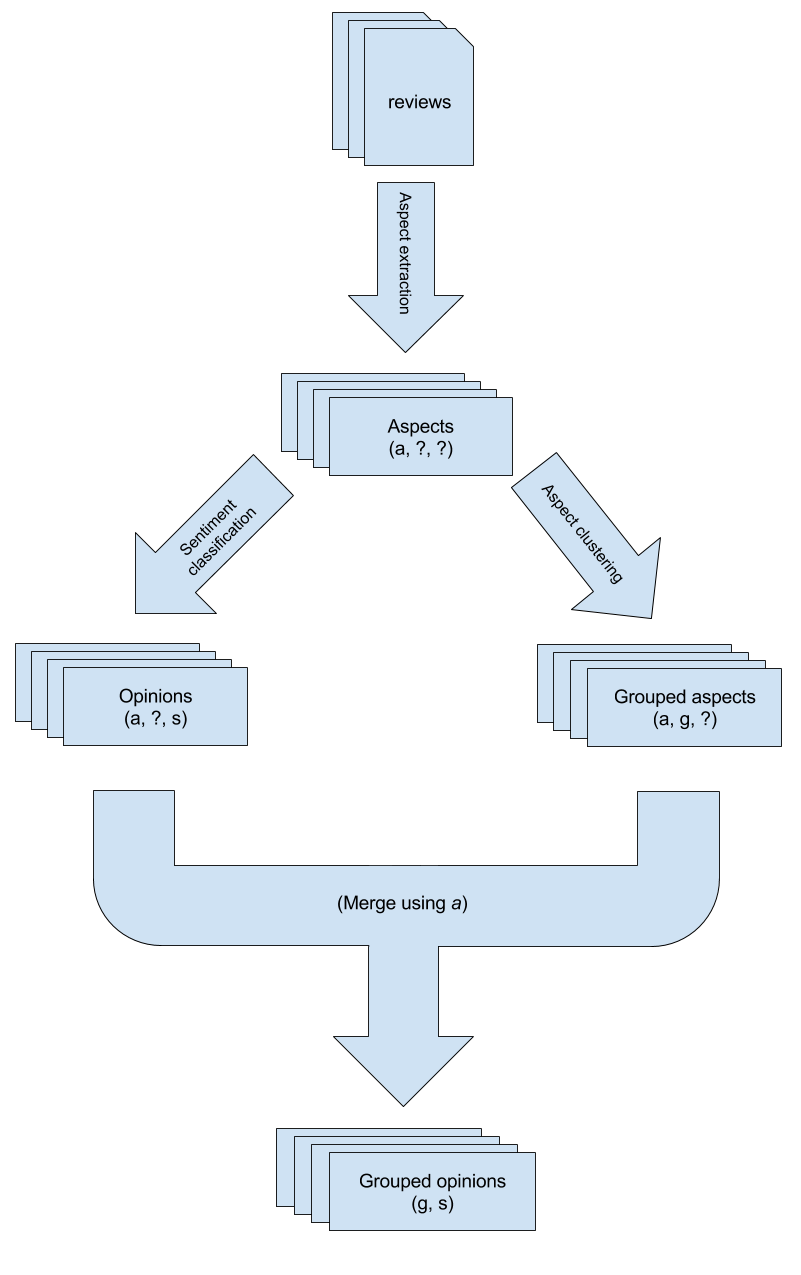
\includegraphics[width=12cm]{overview.png}}
  \caption{High level system overview. Unprocessed review texts processed by the system
    get turned into Grouped opinions; which are partial }
  \label{fig:overview}
\end{figure}



\clearpage

\newpage
\section{Evaluation}
A common way to evaluate information retrieval tasks is \emph{precision} and \emph{recall}. Together they evaluate a systems ability to retrieve results, by evaluating the capacity to exclude irrelevant results, and include relevant results, respectively.

\subsection{Precision}
Precision is a measure of what fraction of retrieved results are considered relevant or correct.

It is defined as follows:
\begin{equation} \label{eq:precision}
Precision = \frac{\text {correctly classified}}{\text{correctly classified} + \text{incorrectly classified}}
\end{equation}

\subsection{Recall}
In this work, confidence thresholds are used to examine whether better results can be achieved by
allowing the classifiers answer \texttt{UNKNOWN} for difficult cases. These answers are not included in
the precision denominator, as they are not considered to be classified.
Instead \emph{recall} is introduced to mean the fraction of results that classifiers gave an answer for:

\begin{equation} \label{eq:recall}
Recall = \frac{\text {classified}}{\text{classified} + \texttt{UNKNOWN}\text{s}}
\end{equation}

%\subsection{Perplexity}






\chapter{Aspect extraction}

\section{Problem definition}
Aspect extraction is the task of finding and outputting sentiment carrying expressions
with identified \emph{targets}. A target is either some aspect of the entity that is
subject to the sentiment, or the entity in its entirety. E.g. in the sentence
\emph{``I like \textbf{this place} even though \textbf{the service} isn't great''},
there are two opinions with one (highlighted) target each; the entity itself, and the
service-aspect of the entity.

Aspect extraction then is a typical information retrieval task, and thus methods
(including evaluation) can be recognized from data mining- and other information retrieval tasks.
In general, there are four approaches to aspect extraction\cite[chapter 5.3]{liu2012sentiment}:

\begin{enumerate}
\item Extraction based on frequent nouns and noun phrases
\item Extraction by exploiting opinion and target relations
\item Extraction using supervised learning
\item Extraction using topic modeling
\end{enumerate}
In this work only the first kind is employed, and results will show it sufficiently
effective to motivate focusing on the other problems.

\subsection{A data dependent task}
Like other data extraction tasks, aspect extraction is largely dependent on the data
aspects are being extracted from. Techniques may vary in effectiveness depending
on what domain they are applied to, demographics of review authors,
contextual expectations of the reviewed entity and countless other factors.

Furthermore, even within the same data set, there may be hidden properties on a
per-entity basis. E.g. one could imagine that even on the same review sitem, there would still
be systematic differences between reviews written for a surgeon's instrument
compared to reviews for a toy car.

It is therefore crucial that in the process of aspect extraction, like in other extraction tasks,
to think about what correlations may exist and what bias they may introduce in the extracted data.


\subsection{Candidate extraction vs. pruning}
There are two important definitions in this section,
which together make up the method used in this work:

\emph{Candidate identification} is the task of finding potential aspects in unstructured text.

\emph{Pruning} is the task of excluding irrelevant candidates that from the candidate
identification result set.

The reason why these usually are done separately in sequence is that many common pruning
techniques require the full candidate set when deciding whether to prune.
(Examples are \emph{idf}-scores or plain occurrence counts.)


\section{Related Work}

\subsubsection{Turney (2002)}
In early work, Peter Turney classified sentiment of reviews for \emph{automobiles}, \emph{banks}, \emph{movies} and \emph{travel destinations} with accuracies ranging from 66-84\%, by extracting aspects using predefined POS-patterns, and querying search engines for the co-occurrence between found patterns and the words \emph{``excellent''} and \emph{``poor''}.

\subsubsection{Hu, Liu (2004)}
In ``Mining Opinion Features in Customer Reviews'', reviews are POS-tagged and common data
mining methods are used to on to find patterns that extract features(aspects).
Sentiment classification is mentioned, but those results are presented in a subsequent paper.

\subsubsection{Liu, Hu and Cheng (2005)}
In ``Opinion observer: analyzing and comparing opinions on the web'' a visualization interface
for review analysis comparison is proposed.

In this work, aspects are extracted by mining data for POS-patterns that indicate aspects,
rather than mining aspects directly. The same rule-mining is used to find mapping for implicit aspects.

\newpage
\section{Extracting aspects}
A simple aspect extractor was developed. Given a review, the extractor used the
POS-tagger in nltk\cite{nltk} and compared the text to a series of predefined grammatical patterns.

These patterns were aquired during the annotation described in section \ref{subsec:getting_data}.
Each annotated aspect also included its POS-pattern, so reoccuring patterns were
examined for candidate identification. They are listed in table \ref{tab:used_pos}.

\newcommand{\ExtrPatOne}{\texttt{<NNS?><VB.?>+<JJ.?>+}}
\newcommand{\ExtrPatTwo}{\texttt{<NNS?><VB.?>+<RB.?><JJ.?>}}

\begin{table}[t]
  \centering
  \begin{tabular}{| l | l |}
    \hline
    \textbf{Pattern} & \textbf{Sample sentence}\\ \hline
    &\\

    \hline
  \end{tabular}
  \caption{Patterns used in entity extraction}
  \label{tab:used_pos}
\end{table}

\section{Results}

\begin{figure}[h]
  \centering
  \begin{tikzpicture}

  \begin{axis}[
      xlabel={Found aspects},
      ylabel={No. reviews},
      ybar, ymin=0, %3ymax=9999,
      %bar width=20pt,
      xtick=data,
      %x tick label style={rotate=45,anchor=east},
      xticklabels from table={data/extraction_counts.csv}{found},
      xticklabel style={text height=1.5ex},
      ymajorgrids=true,
      grid style=dashed,
      legend pos=north east,
    ]
    \addplot table [x expr=\coordindex, y=count]{data/extraction_count1.csv};
    \addplot table [x expr=\coordindex, y=count]{data/extraction_count2.csv};
    \addplot table [x expr=\coordindex, y=count]{data/extraction_count_both.csv};
    \legend{
      \ExtrPatTwo,
      \ExtrPatOne,
      Both patterns,
      }
  \end{axis}
  \end{tikzpicture}
  \caption{Distribution of number of extracted aspects per review}
  \label{fig:extr_count}
\end{figure}



Out of 10'000 reviews, in total 12'246 aspects were found, which works out to an average of around 1.2 aspects per review. Figure \ref{fig:extr_count} shows the distribution of reviews and the number of found aspects. Note that the graph does not show how many aspects were found, but in how many reviews a certain number of were found.

\section{Discussion}

On average, just above one aspect per review is found, which may not sound like a lot, but for entities with lots of reviews it may be enough. Later in this work when we study aspect clustering, figure \ref{fig:cat_count} will show that the least common category, \emph{value}, represents around 10\% of the aspects, for a reviewed entity with 300 reviews then, around 35 opinions can be expected, which should be enough for a conclusion. In practice, review comparisons would likely be done for business chains which can easily have 10'000 reviews, which is why in this work this simple method was deemed sufficient.

To make conclusions more impartial, it might be a good idea to only allow one opinion per aspect from each review. Arguably one reviewer mentioning a bad service experience ten times should not be valued the same as positive mentions from ten reviewers. Ideally, some average of all sentiments for  each aspect in one review should probably be used when summarizing results, but the aspect extraction task may know what category found aspects belong to. If this is a concern a definite lower bound can still be estimated by allowing at most one aspect per review, which effectively would eliminate this risk at the cost of about half of all found aspects.

Another problem that is harder to mitigate is presented by the method itself; basing a conclusion on aspects extracted from a single pattern effectively concludes what reviewers \emph{using language with that pattern} think of something. Adding more patterns would mitigate this risk, but I think the best way to circumvent this problem would be to use at least two fundamentally different methods in combination, such as including a supervised learner.

%patterns by trial and error

%\section{Further improvements}


\chapter{Sentiment Classification}
Sentiment classification is the problem of deciding whether sentiment in a sentence is positive, negative or neutral\cite{nlp_book}. Being a central part of sentiment analysis it can also done on the same three levels: Document level, sentence level and aspect level.

Sentiment classification can be a classification- or regression analysis problem\cite{liu2012sentiment}, depending on whether results are expected to be discrete class-labels or a continuous measures of positively. In this report the discrete classification definition will be used unless otherwise specified.

\section{Language modeling}

\subsection{\ngram s}
\ngram~modeling is a versatile, robust and widely used method of modeling languages. Typically the model consists of, for some $n$, all $n$-length sub-sequences of a longer sequence (i.e. one or many documents). Each unique sub-sequence is then referred to as a \ngram, and \ngram s of length \emph{1,2,3} are referred to as \emph{unigrams, bigrams} and \emph{trigrams}, respectively\cite{ngrams}.

Frequencies, counts and occurrences of \ngram s have been used in language modeling\cite{chen_goodman}, text categorization\cite{ngrams}, \todo

As an example, the word-\emph{bigrams} for the sentence \emph{``Languages are fun''} are:
\begin{quote}
  \vspace*{0.1cm}
  \centering
\emph{``\$ Languages''}, \emph{``Languages are''}, \emph{``are fun''}, and \emph{``fun \$''}
\end{quote}
where \emph{\$} is a token meaning the start/end of sentence.

Although \ngram~modeling can be applied to virtually any kind of sequence, this report henceforth will refer exclusively to \ngram s consisting of words.

\subsection{\ngram~language modeling}
If the probability of a word's occurrence in a sentence $P$ is known (e.g. estimated using a corpus), then the probability of a sentence $s$ can be modeled the following way with \emph{unigrams}:

\begin{equation} \label{eq:unigram_chain_prob}
P(s) \approx P(w_1) P(w_2) \dots P(w_n) =\prod_{w_i \in s}P(w_i)
\end{equation}
Similarly, if modeled with \emph{bigrams}:

\begin{equation} \label{eq:bigram_chain_prob}
P(s) \approx P(w_2 | w_1)P(w_3 | w_2) \dots P(w_n | w_{n-1}) = \prod_{w_i \in s}P(w_i|w_{i-1})
\end{equation}
Where $P(w_b | w_a)$ is some probability estimate of a word being $w_b$, provided that the previous word was $w_a$. (Modeling the probability of a word's occurrence solely on previous element(s) in the sequence is know as \emph{the Markov assumption}.) It should be clear that good \ngram~modeling then is about finding a $P$-function that estimates reality well.

A naive \gls{MLE} of a sentence $s$ could be defined something like this:
\begin{equation} \label{eq:bigram_mle}
P(w_i|w_{i-1}) = \frac{c(w_{i-1}\,w_i)}{\sum_{w} c(w_{i-1}\, w_*)}
\end{equation}

Here the number of occurrences where the word $w_{i-1}$ follows $w_i$ (as provided by the count function $c$) are normalized by the number of occurrences where $w_{i-1}$ is followed by any word $w_*$, or in other words the fraction of this particular bigram out of all bigrams with the same first word.

\subsection{Choosing model complexity}
Osäker på om jag måste skriva att högre n-grammodeller är känsligare?
\loremipsum

\section{Smoothing language models}
A common problem when statistically modeling based on existing data,
is how the model should handle previously unseen entities.
Since human language is virtually infinite, even reasonable sentences are innumerable,
and thus handling unseen data is a requirement for good performance.

As can be seen in equation \ref{eq:bigram_mle}, the \gls{MLE} of entities unseen in
training data would per definition be assigned a zero probability, which in turn makes
the chain model(eq.~\ref{eq:bigram_chain_prob}) assign a zero probability to the entire
sentence\cite{chen_goodman}.

Smoothing is a means of improving models with limited data samples.
It can mitigate the problem of unseen data,
but also makes for better estimations of rare entities.

\subsection{Additive smoothing}
One of the most basic smoothing techniques called \emph{additive smoothing},
or \emph{Lidstone Smoothing}, introduces a constant $\alpha$ which ensures
non-zero probabilities\cite{chen_goodman}:
\begin{equation} \label{eq:additive_smoothing}
P_{add}(w_i|w_{i-1}) = \frac{c(w_{i-1}\,w_i)+\alpha}{\sum_{w} \big[c(w_{i-1}\, w_*)+\alpha\big]}
\end{equation}
where $0 < \alpha \leq 1$ is commonly used. The case when $\alpha=1$ is also called \emph{Laplace smoothing}\cite{nlp_book}.


\subsection{Interpolated smoothing}
Additive smoothing addresses unseen data, there are other models that give more accurate estimations.

\emph{Interpolated smoothing} is a way of combining models of various complexities,
in this case multiple \ngram~models with different lengths. In interpolation, the probabilities of each model are summed, usually weighted so higher complexity models are given more influence\cite{chen_goodman}.
Below is an example of what most interpolated smoothing approaches look like for bigrams:
\begin{equation}\label{eq:interpolated_smoothing}
  P_{inter}(w_i|w_{i-1}) =
  \lambda_2 P(w_i|w_{i-1}) + \lambda_1 P(w_i)
\end{equation}

where $\lambda_1, \lambda_2$ are weights dividing influence between models, and $\lambda_1 + \lambda_2 = 1$.
In my experiments $\lambda_1 = \lambda_2 = 0.5$ yielded the best results, but this is data dependent.

Interpolated smoothing techniques mitigate the trade-off between complex models with higher accuracy and simpler models that generalize well. If a queried bigram does not exist in training data at all, the first term will effectively equal zero, and the estimate will be the one of a individual unigram model times a reducing factor.

The above can easily be generalized to include arbitrarily high \ngram~models by extending the number of terms to match the highest included model.

%\subsection{Modified Kneser-Ney smoothing}
%One of the most commonly used modern smoothing methods is \emph{interpolated Kneser-Ney smoothing},
%or \emph{Modified Kneser-Ney smoothing}\cite{nlp_book}, which incorporates two additional intuitions:
%
%Firstly, since higher order models have lesser total counts in the denominator,
%even few occurences will have high probabilities compared to lower order models.
%This is addressed by subtracting a \emph{discounting }
%
%
%The first one is that common features with high counts already have high probabilities, so subtracting a small value from counts will affect uncommon features that the model is insecure about and thus for those features give more influence to the lower order models. This is called \emph{absolute discounting}\cite{npl_book}. \emph{Modified Kneser-Ney smoothing}, as opposed to the model originally proposed by\emph{Kneser-Ney}, uses four different constants depending on the occurrence count it is penalizing.
%
%The second intuition is that just as lower order models are given higher influence when the higher models have less confidence, lower order models should not be consulted when higher order models estimate well. \emph{TODO: Example: With many occurrences of  ``San Francisco'', where ``Francisco'' only occurs after ``San'', the unigram model will overestimate the sentence ``In the park I got bitten by a Francisco''}.

\section{Classification methods}
The previous section introduces language modeling, which is used to give the probability of a sentence.
Classification can without much effort be reduced to language modeling, by training one model per class and
selecting the model assigning the highest probability. This is in fact what many common classifiers do.
(In fact, due to the assumtion that \ngram~occurrences are independent, eq. \ref {eq:bigram_mle}
could be viewed as a Naive Bayes classifier with only one class(prior=1).)



\subsection{Scikit-learn and other classification methods}
Scikit-learn\cite{scikit-learn} is a collection of machine learning implementations in Python, ready to use ``out of the box''.

The following methods were examined in this work:

\begin{table}[h]
  \centering
  \begin{tabular}{ r l }
    \textbf{Module name} & \textbf{Explanation}\\
    GaussianNB (\texttt{GNB}) & Gaussian distributed prior Naive Bayes classifier.\\
         %& No smoothing (Gaussian prior).\\
    MultinomialNB (\texttt{MNB}) & Multinomial distributed prior Naive Bayes classifier. \\
         %& Additive smoothing.\\
    BernoulliNB (\texttt{BNB})& Bernoulli distributed prior Naive Bayes classifier.\\
         %& Additive smoothing.\\
    LogisticRegression (\texttt{LR}) & \\
    SGDClassifier (\texttt{SGD}) & \\
    SVC (\texttt{SVC})& \\
    LinearSVC (\texttt{LSVC}) & \\
    NuSVC (\texttt{NSVC})& \\
  \end{tabular}
  \caption{todo}
  \label{tab:scikit_classifiers}
\end{table}

Section \ref{tab:clf_results} shows the individual classifier performances, and based on these results,
\todo were selected when developing an ensamble classifier. To classify, the ensamble consulted each of
the included classifiers individually, and selected the class with the highest probability sum(using
$p=0.75$ \footnote{Selected using binary search between 0.5 and 1.}
for classifiers based on other concepts than probabilty, like SVCs and Logistic Regression).

%Confidence was defined as the average 


\newpage
\section{Related work}
Various approaches to sentiment classification exist, where approaches can generally be categorized as either grammatical\cite{todo} or statistical\cite{todo}. This sections aims to give some insight into what has been previously done in the field.

\subsubsection{Chen, Goodman (1996)}
In the thorough study ``An empirical study of smoothing techniques for language modeling.'' smoothing is
thoroughly studied with regard to language modeling. Furthermore, a novel variation of an existing
smoothing technique is introduced, \emph{Modified Kneser-Ney}-smoothing, which outperforms other
smoothing methods to date.


\subsubsection{Turney (2002)}
In early work, Peter Turney classified sentiment of reviews for \emph{automobiles}, \emph{banks}, \emph{movies} and \emph{travel destinations} with accuracies ranging from 66-84\%, by extracting aspects using predefined POS-patterns, and querying search engines for the co-occurrence between found patterns and the words \emph{``excellent''} and \emph{``poor''}.

\subsubsection{Hu, Liu (2004)}
In ``Mining Opinion Features in Customer Reviews'', reviews are POS-tagged and common data mining methods are used to on to find patterns that extract features(aspects). Sentiment classification is mentioned, but results are presented in a subsequent paper.

\subsubsection{Hu, Liu (2004)}
In ``Mining and summarizing customer reviews'', previous work by the same authors is extended with sentiment classification to produce product summaries. Sentiment is classified by looking for \emph{sentiment words} predefined as positive or negative or their synonyms/antonyms using WordNet. Their method also searches for nearby \emph{negation words}, which if found, simply negate the outcome of the classification.

Finally a summary is produced, but this process is very briefly described, and is without evaluations. To my understanding, opinions are solely grouped on the lemmatized form of explicit aspects.


\pagebreak
\section{Experiment setup}

\subsection{Available data}

\subsubsection{Training data: Yelp academic data set}
From the Yelp academic data set\footnote{https://www.yelp.com/dataset\_challenge/},
reviews were randomly selected from 900940 positive reviews (rated 5/5)
and 260492 negative reviews(rated 1/5). Most reviews consist of more than one sentence.

Based on an underlying assumption that positive reviews consist predominantly of more
positive than negative language, and vice versa for negative reviews,
sentences were labeled as positive or negative depending on what review they originated from.

These reviews were used to train classifiers.

\subsubsection{Evaluation data: Sentiment labeled sentences}
Yelp has a data set with 3216 positive and 1271 negative sentences labeled
according to their sentiment towards the the business in general.

These were used to evaluate the sentiment classifiers.

\subsection{Studied classifiers}
To examine the effects of varying \ngram models and smoothing,
three \ngram~classifiers with additive smoothing were developed, based on the
probability definition in equation \ref{eq:additive_smoothing}.

The classifiers were trained on 4'000 sentences from postive reviews
and another 4'000 sentences from negative reviews.
As features, up to the 30'000 most common \ngram s were used\footnote{As table
  \ref{tab:found_ngrams} shows, the unigram model only produces 8772 \ngram s,
  in which case all of them were used.}.


Two more classifiers were developed with interpolated smoothing, 

The third classifier combines the above classifiers,
\emph{interpolated} as suggested in eq. \ref{eq:interpolated_smoothing}, with
$(\lambda_2=\lambda_1=0.5)$.

%Finally, for reference of what a production system can look like, Yelp's production classifier was included in results. It is based on a \emph{Modified Kneser-Ney}-smoothed language model.


\newpage
\section{Results}

\begin{figure}[h]
  \centering
  \begin{tikzpicture}
    \begin{axis}[
        xlabel={Recall (normalized)},
        ylabel={Precision},
        xmin=0, xmax=1,
        %ymin=0.4, ymax=1,
        %xtick={0,20,40,60,80,100},
        %ytick={0,20,40,60,80,100,120},
        legend pos=north east,
        ymajorgrids=true,
        grid style=dashed,
      ]
      %\addplot table [x=r, y=p]{data/sent_yelp_pr.csv};
      \addplot table [x=r, y=p]{data/sent_new_unigram_pr.csv};
      \addplot table [x=r, y=p]{data/sent_new_bigram_pr.csv};
      \addplot table [x=r, y=p]{data/sent_new_trigram_pr.csv};
      \addplot table [x=r, y=p]{data/sent_new_interpol_12_pr.csv};
      \addplot table [x=r, y=p]{data/sent_new_interpol_123_pr.csv};
      \legend{
        %yelp..,
        \texttt{Unigram},
        \texttt{Bigram},
        \texttt{Trigram},
        \texttt{Interpol2},
        \texttt{Interpol3},
      }
    \end{axis}
  \end{tikzpicture}
  \caption{Sentiment classifier precision vs. recall. Each dot represents a
    10\% increase in confidence threshold (starting with 1.0 at the left).}
  \label{fig:sent_pr_curve}nn
\end{figure}


\subsection{Introducing confidence thresholds}
Figure \ref{fig:sent_pr_curve} shows how the \emph{interpolated} classifiers have
consistently better performance than the additively smoothed classifiers.
More specifically \texttt{interpol3} also outperforms \texttt{interpol2}, which
not surprisingly means that adding another model to the interpolation improves results.

It can also be seen that lower order models generalize better, as when required to
classify all samples, they perfom better than higher order models, whereas the higher
order models exhibit higher confidence in a few samples and in turn have higher
precision with lower recall.


\newpage

\subsection{Per class classification}
\begin{figure}[h]
  \centering
  \begin{tikzpicture}

  \begin{axis}[
      %title={Classifier performance per category},
      %xlabel={Categories},
      ylabel={Fraction of correctly classified},
      ybar, ymin=0.5,
      %bar width=20pt,
      xtick=data,
      x tick label style={rotate=45,anchor=east},
      xticklabels from table={data/sent_unigram.csv}{l},
      xticklabel style={text height=1.5ex},
      ymajorgrids=true,
      grid style=dashed,
      legend pos=south west,
    ]
    \addplot table [x expr=\coordindex, y=p]{data/sent_yelp.csv};
    %\addplot table [x expr=\coordindex, y=p]{data/sent_unigram.csv};
    %\addplot table [x expr=\coordindex, y=p]{data/sent_bigram.csv};
    %\addplot table [x expr=\coordindex, y=p]{data/sent_interpol.csv};
    \legend{\ysc, unigram, bigram, interpolated}
  \end{axis}
  \end{tikzpicture}
  \caption{Perfomance of classifiers per class. No thresholds(recall=1)}
  \label{fig:sent_per_cat}
\end{figure}


\begin{table}[t]
  \centering
  \begin{tabular}{| c | c |}
    \hline
    \textbf{Model} & \textbf{Found \ngram s}\\ \hline
    Unigram&8772\\
    Bigram&55295\\
    Trigram&92569\\
    \hline
  \end{tabular}
  \caption{Number of unique \ngram s for different \ngram~lengths}
  \label{tab:found_ngrams}
\end{table}

\subsection{Per class}
todo

\subsection{Notable examples}
TODO: Table with number of failures per classifier.

Examples of where \ysc~succeeds but my classifiers fail, use to speculate about smoothing.


\newpage
\section{Discussion}

One of the most imporant results shown in Figure \ref{fig:sent_pr_curve} is that feature selection is not in itself deteriming performance.  Which can be concluded from the interpolated classifier being supperior, and from the unigram and bigram model comparison depending on recall.

The fact that the unigram model performs better than the bigram model at full recall, but that the bigram model is better at confidence $>80\%$, indicates that the unigram model generalizes better and that the bigram model has higher confidence in results that align well with the model, which confirms premises that has motivated previous studies of smoothing.

It should be noted that the comparison between \ysc~and the other models is unfair, since the \ysc~has been trained on more data and has been rigurously tested and reviewed. It is solely included to give perspective on performance of the simpler models.

Figure \ref{fig:sent_per_cat} shows all classifiers have a slight bias towards the positive class despite down-sampling training data to be equal. I believe that this is due to positive reviews being more expressive of sentiment. It could arguably be a desired property for real world applications as real data has an even larger positive bias, which makes statistical models align better with reality. There may also be a social benefit of this positive bias.


% logical negation might clash with bi-gram model
% introducing neutral-class
% actually training to identify positive reviews, not positive statements



\subsection{Difficulties}
\subsubsection{Subjective and objective sentiments}
Sentiment can be derived in various ways. \emph{``I disliked the taste of my coffee''} is an example of a sentence subjective sentiment. Subjective sentiments may per definition not apply to everyone.

Sentiment can also be derived from objective sentences: \emph{``the toilet seat was broken''} clearly implies negative sentiment as \emph{broken} is an unquestionably negative property for a toilet. Most sentences are somewhere in between subjective and objective, e.g. the sentence ``the portion size was small'' is of objective nature, but holds a subjective definition of \emph{small portion size}.

Just as objective sentences can hold sentiment, subjective sentences may not, as ``I thought the ''


\subsubsection{Further work}


% ``I would've most likely ordered dessert if I had more time and if the waitress was not too busy''
% ``we had the deep fried scallops ($14) nice and juicy.''
% ignored comparative sentiments
% ``The dining room with  low lighting is casual with comfortable booths and tables and a separate lounge area with more seating to watch sports''
% ``The', 'menu', 'offers', 'sandwiches', ',', 'appetizers', ',', 'steaks', ',', 'seafood', ',', 'chicken', ',', 'ribs', ',', 'prime', 'rib', ',', 'pasta', ',', 'salads', ',', 'homemade', 'soups', ',', 'and', 'desserts',
% Good food at reasonable prices
% I like beef with potatoes on the side
% I love steaks


% Comparative opinions, PRUNE.


% =========================================================================================================



\chapter{Aspect Clustering}
So far this work has introduced methodology for extracting aspects from text and classifying their sentiments, which introduces a new problem: How can these aspects with known sentiments be combined into an adequate summary?

The first and most important observation is that even if we find a statement and accurately identify it as a positive mention on something, it is not enough to merit a conclusion. Opinions are per definition subjective, and should individually be considered unreliable. However, as the number of processed opinions increase, so does confidence in conclusions that are based on them.

As a consequence, four positive mentions of ``steak'' may not be enough for a conclusion, but in combination with positive mentions on ``chicken'', ``turkey'',  and ``meatballs'' one may be able to conclude positive the common \gls{superword} \emph{meats}. Or if more confidence is required, ``salads'' may be included under the \gls{superword} \emph{food}, and so on.

This is task is defined as \emph{aspect clustering}, or in some work \emph{aspect grouping}.


\subsection{Skewed data}
\label{subsec:bias}
When dealing with real world data, it is possible that some classes in classification problems are more
common than others. This has been shown to have consequences both in Bayesian classifiers\cite{rennie2003bias}
and Support Vector Machines\cite{svm_bias}, where both have been shown to favor majority
classes\cite{rennie2003bias, svm_bias}.

Not only classification methods, but also precision measures are affected by skewed data. In binary
classification with evenly distributed classes, a classifier that favors one class to the extreme that it
always chooses the same class, still achieves around 0.5 precision since the number of true positives
would equal the proportion of the favored class\footnote{This is in fact be the worst possible result
in the binary case, since any classifier performing consistently worse could be modified to return the
opposite and thus have the inverse precision.}. This also illustrates that there is a dependency between
precision of biased classifiers and distribution of classes in test data.

A commonly employed and simple way to solve problems with disproportionate data altogether is to exclude all but an equal amount from each class to artificially balance the class distribution, also sometimes referred to as \emph{down-sampling}\cite{provost2000machine}. This could pose a problem if data is very skewed, as this means that the required amount of data is effectively multiplied by the fraction of the least common class. However, in this work the data was not skewed enough to consider more sophisticated other approaches.

Although artificially balanced evaluation data eliminates bias in evaluations, which makes evaluations between classifiers more comparable, it also reduces the amount of entries used for evaluation, which makes evaluations less informed. Therefore this report will evaluate unscaled data once classifiers have been verified to be reasonably unbiased in a per class comparison.

\section{Experiment setup}
For these experiments, Yelp reviews from the \category were manually annotated in various ways.

\numAnnotated~sentences were manually annotated on the sentence level and divided into three parts: Training, testing and evaluation. During development the first two parts of the data-set were made available, whereas the evaluation set of sentences was kept separately to ensure reliable results. To ensure impartialness of methods and increase reliability of results, the only output allowed from the evaluation data set was strictly restricted to summaries of results (i.e. no individual results were presented with their outcome)\ifhasStudiedFailures, except for when failing instances were explicitly studied after method development was finished\fi.

\newpage
\subsection{Getting data}
\label{subsec:getting_data}
\begin{figure}[h]
  \centering
  \fbox{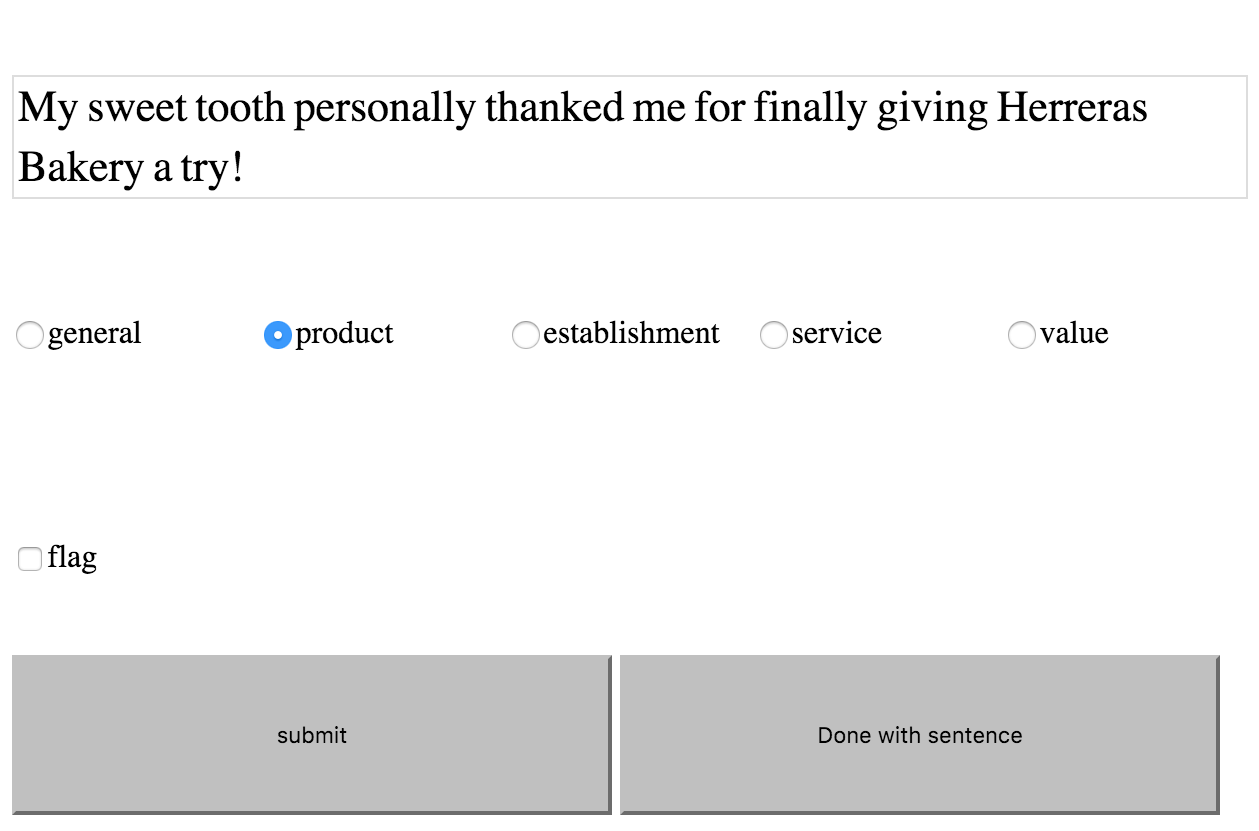
\includegraphics[width=10cm]{annotate_sentence.png}}
  \caption{Sentence level annotation interface}
  \label{fig:annotate_sentence}
\end{figure}

\begin{figure}[h]
  \centering
  \fbox{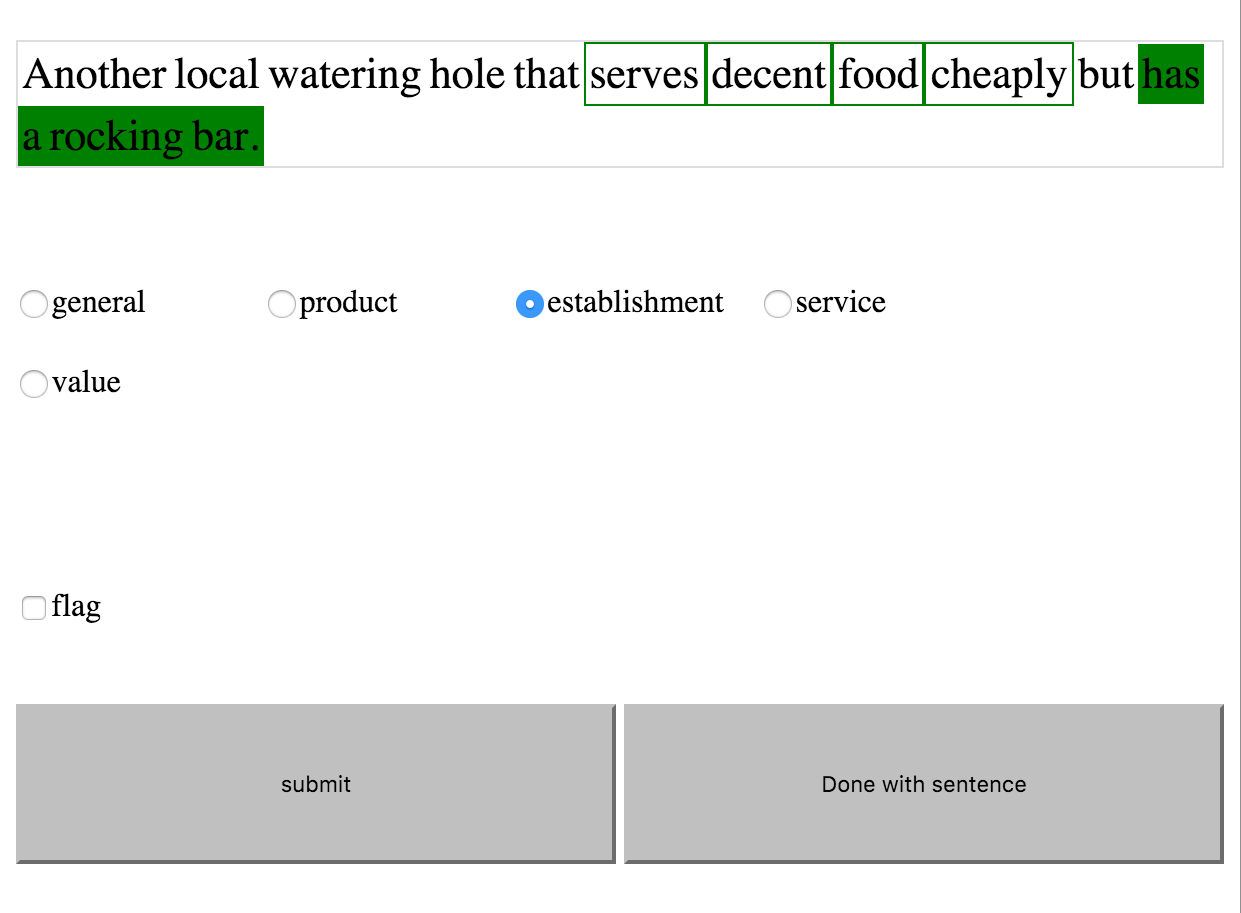
\includegraphics[width=10cm]{annotate_aspect.png}}
  \caption{Aspect level annotation interface. Allows selection of aspects by marking a series of words(dark green). Since a sentence can hold more than one aspect, once an aspect has been submitted, the same sentence is kept and another aspect can be selected(a green border is left to indicate a previous submission).}
  \label{fig:annotate_aspect}
\end{figure}

Figures \ref{fig:annotate_sentence} and \ref{fig:annotate_aspect} show the interface that was developed to annotate on the \emph{sentence level} and \emph{aspect level} respectively. This simple web-interface was served by a local web server and could be accessed by multiple users simultaneously.


\begin{figure}[t]
  \centering
  \begin{tikzpicture}

  \begin{axis}[
      %title={Classifier performance per category},
      %xlabel={Categories},
      ylabel={Number of aspects},
      ybar, ymin=0,
      %bar width=20pt,
      xtick=data,
      x tick label style={rotate=45,anchor=east},
      xticklabels from table={data/category_distribution.csv}{category},
      xticklabel style={text height=1.5ex},
      ymajorgrids=true,
      grid style=dashed,
      legend pos=north east,
    ]
    \addplot table [x expr=\coordindex, y=count]{data/category_distribution.csv};
  \end{axis}
  \end{tikzpicture}
  \caption{Number of annotated sentences per category}
  \label{fig:cat_count}
\end{figure}


\newpage

\section{Aspect clustering}
\subsection{Using graph search}
Based on the observation that there are usually key words in a sentence with lexicographical connection to the desired category, an alternative approach to traditional classification is proposed. This is motivated since classification models need pure training data to achieve good results. The idea is to use a lexicon of known word relations to find a path from a query word to one of few word senses with predefined category label, and assign the query word the same label.

Figure~\ref{fig:baklava_lex} shows an example of this premise in action, where the word relations involved in finding the word ``baklava'' were used, and that it is closer to \emph{product} than \emph{establishment}.

\subsubsection{The algorithm}
A \gls{BFS}(BFS) is conducted from the initial category word senses, defined in table \ref{cat_words}. For each word, neighboring word senses are acquired using word relations defined by \gls{jaws}). Each word sense is also mapped to its source category in this process to allow for quick look-ups.

This method to categorize individual words, can then be extended to categorize full sentences using heuristics.

\subsubsection{Voting heuristic}
The heuristic is given a sentence, and is supposed to decide on a cluster for the entire sentence. To do this, it can use the above described setup to query for the category of an individual word sense. Since word senses can consist of more than one word, e.g. ``happy hour'', the heuristic iteratively searches the sentence word senses, decreasing in length, starting with the assumption that the full sentence is one word begin.

Next, the map built using the word relation search was queried for the category of each word sense. The result of each query is not only which category, but also the distance $d$ from the word sense to the category. This was then combined into one score using the following scheme:

\begin{equation} \label{eq:heruistic}
  category(s) =
  \underset{k}{\text{argmax}}
  \sum_{w \in s} categoryScore(w, k)
\end{equation}

\begin{equation} \label{eq:heruistic_d}
  categoryScore(w, k) =
  \begin{cases}
    max(d_*) - d_k(w) + 1, & \text{if}\ d_k(w) < d_{\,!k}(w)\\
    0, & \text{otherwise}
  \end{cases}
\end{equation}

where $d_k(w)$ is the distance from the word sense $w$ to its nearest category and $d_*$ is the biggest distance for any word to its nearest category.

This way, a three word sentence with distances $d_A(w_1)=4$, $d_A(w_2)=6$ and $d_B(w_3)=3$, will receive the scores $A=3+1$ and $B=4$, and thus category $A$ would be selected.


\begin{table}[t]
  \centering
  \begin{tabular}{| c | c |}
    \hline
    \textbf{Category} & \textbf{Predefined keywords}\\ \hline
    Establishment & \emph{Furniture, view, music, loud, appearance, clean, location}\\ \hline
    Product & \emph{food, taste, edible}\\ \hline
    Value & \emph{Cheap, price, dollar, buck, lots, bargain}\\ \hline
    Service & \emph{Service, quick, attentive}\\ \hline
  \end{tabular}
  \caption{Categories with their pre-associated key words.}
  \label{cat_words}
\end{table}

\begin{figure}[t]
  \centering
  \fbox{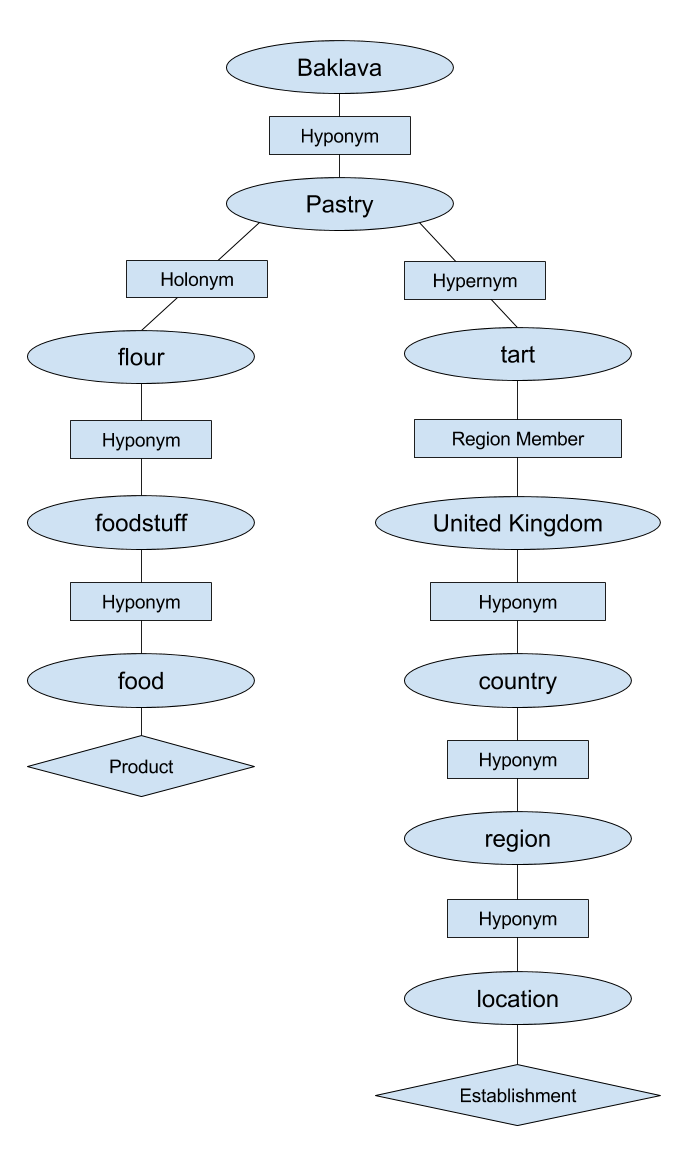
\includegraphics[width=10cm]{img/baklava_lex.png}}
  \caption{Example showing how ``baklava'' could be lexicographically closer to category ``product'' than ``establishment''. Ellipses represent word senses, rectangles the relations between senses, and diamonds predefined categories with a few associated senses (in this case \emph{food} and \emph{location}).}
  \label{fig:baklava_lex}
\end{figure}

\clearpage

% todo: annotations interface screenshot
% todo: num sentences table


\section{Results}

This chapter is laid out as follows: First the individual results for each of the \numClassifierAproaches~classifier approaches are walked through. This gives the reader a chance to better understand section \ref{sec:comparison} where the classifiers are compared.


\subsection{Machine learning classifiers}

\begin{figure}[h]
  \centering

  \begin{tikzpicture}
    \begin{axis}[
        %title={Classifier performance based on data size},
        xlabel={Training data-set size},
        ylabel={Fraction of correctly classified},
        %xmin=0.3, xmax=0.7,
        %ymin=0.25, ymax=0.75,
        %xtick={0,20,40,60,80,100},
        %ytick={0,20,40,60,80,100,120},
        legend pos=north west,
        ymajorgrids=true,
        grid style=dashed,
      ]
      %\addplot table [x=n, y=p]{data/data_size_unigram.csv};
      \addplot table [x=n, y=p]{data/data_size_unigram_balanced.csv};
      \addplot table [x=n, y=p]{data/data_size_bigram.csv};
      \legend{
        %biased unigram,
        unigram,
        bigram
      }
    \end{axis}
  \end{tikzpicture}
  \caption{Sentence classification performance based on training data size}
  \label{fig:data_size}
\end{figure}


As expected, figure \ref {fig:data_size} shows that increased quantities of training data quickly yield improved results. This increment appears approximately linear, up to some point where it is expected to converge. Interesting is how the simpler unigram method quickly outperforms the bigram model, but that the bigram model sees very steady increment.

\pagebreak

\subsection{Per class classification}
\begin{figure}[h]
  \centering
  \begin{tikzpicture}

  \begin{axis}[
      %title={Classifier performance per category},
      %xlabel={Categories},
      ylabel={Fraction of correctly classified},
      ybar, ymin=0,
      %bar width=20pt,
      xtick=data,
      x tick label style={rotate=45,anchor=east},
      xticklabels from table={data/per_category_unigram.csv}{n},
      xticklabel style={text height=1.5ex},
      ymajorgrids=true,
      grid style=dashed,
      legend pos=north east,
    ]
    \addplot table [x expr=\coordindex, y=p]{data/per_category_unigram.csv};
    \addplot table [x expr=\coordindex, y=p]{data/per_category_unigram_unbalanced.csv};
    \addplot table [x expr=\coordindex, y=p]{data/per_category_bigram.csv};
    \addplot table [x expr=\coordindex, y=p]{data/per_category_bigram_unbalanced.csv};
    \legend{balanced unigram, unbalanced unigram, balanced bigram, unbalanced bigram}
  \end{axis}
  \end{tikzpicture}
  \caption{Balanced vs. unbalanced classifier comparison. No confidence threshold was set in this experiment: recall was 1.}
  \label{fig:per_cat}
\end{figure}


%\begin{figure}[h]
%  \centering
%  \begin{tikzpicture}
%
%  \begin{axis}[
%      %title={Classifier performance per category},
%      %xlabel={Categories},
%      ylabel={Fraction of correctly classified},
%      ybar, ymin=0,
%      %bar width=20pt,
%      xtick=data,
%      x tick label style={rotate=45,anchor=east},
%      xticklabels from table={data/per_category_unigram.csv}{n},
%      xticklabel style={text height=1.5ex},
%      ymajorgrids=true,
%      grid style=dashed,
%      legend pos=north east,
%    ]
%    \addplot table [x expr=\coordindex, y=p]{data/per_category2_unigram.csv};
%    \addplot table [x expr=\coordindex, y=p]{data/per_category2_bigram.csv};
%    \legend{balanced unigram, unbalanced unigram, balanced bigram, unbalanced bigram}
%  \end{axis}
%  \end{tikzpicture}
%  \caption{Percat2}
%  \label{fig:per_cat}
%\end{figure}

Section \ref{subsec:bias} introduced bias in data, along with some of its consequences, which motivated a more detailed study of classifier results on a per class basis. Figure \ref{fig:per_cat} illustrates how classifiers trained on balanced training data perform much more consistent between classes.

Comparison between the balanced/unbalanced versions of the classifier models show that, as expected, there seems to be bias towards the more frequent $product$-class and respectively against the infrequent $value$-class.

It can also be seen that the bigram model is performing poorly for all labels except the \emph{product} class, but the reader is urged to note that this is a consistency between the balanced and unbalanced version of the model.

\newpage

\subsection{Introducing confidence thresholds}
\begin{figure}[h]
  \centering
  \begin{tikzpicture}
    \begin{axis}[
        %title={Classifier performance based on data size},
        xlabel={Recall},
        ylabel={Precision},
        %xmin=0.5, xmax=1,
        %ymin=0.4, ymax=1,
        %xtick={0,20,40,60,80,100},
        %ytick={0,20,40,60,80,100,120},
        legend pos=south west,
        ymajorgrids=true,
        grid style=dashed,
      ]
      \addplot table [x=r, y=p]{data/pr_unigram.csv};
      \addplot table [x=r, y=p]{data/pr_bigram.csv};
      \legend{
        unigram,
        bigram
      }
    \end{axis}
  \end{tikzpicture}
  \caption{Precision vs. recall created varying a confidence threshold}
  \label{fig:pr_curve}
\end{figure}


Figure \ref{fig:pr_curve} shows the expected precision/recall trade-off for the aspect cluster classifiers. Readers should be reminded that each measurement was done on differently balanced training data, which likely accounts for inconsistencies in the curves.

\newpage

\section{Graph-search classifier}
The graph search found a total of 78'844 word senses.



\section{Comparison of classifiers}
\label{sec:comparison}

\begin{table}[h]
  \centering
  \pgfplotstabletypeset[
    columns={method,p,r},
    col sep=comma,
    every head row/.style={after row=\midrule},
    columns/method/.style={string type,column type=l, column name=Classifier},
    columns/p/.style={precision=3, column type=l, zerofill, column name=Precision},
    columns/r/.style={precision=4, column type=l, column name=Recall},
  ]{data/general_aspect.csv}

  \vspace{0.4cm}\caption{Result summary}
  \label{general_asp}
p\end{table}


\section{Discussion}
As the results show, it is in fact possible to categorize aspects using a lexical database. What is particularly interesting about this result is that the heuristic is unsupervised.

There are however a few reasons why the results should be interpreted with caution:

I believe my limited amount of data to have much influence over my results. As figure \ref{fig:data_size} illustrates, neither machine learning classifier appears ``saturated'', and would most likely have benefited from more annotated aspects.

Another important thing to keep in mind about my results are that with such a small data-set, there is a risk of methods becoming too specific toward the training data. This is often discussed in statstical modeling as \emph{``overfitting'' }, but the same phenomenon can also appear with heuristics. I believe that some aspects of my data make this heurisic perform better than it would in general.



%todo reasons:
% small data-set, might be overfitted?

% becomes easier with aspect-word only?

% indata probably works for you

% ``place is really small and seemed kinda dirty''


%\chapter{Conclusions}
%\section{Aspect clustering}

\chapter{Conclusions}
This report has introduced problems and basic approaches known to work for opinon mining.

\subsection{Sentiment classification is not only about feature selection}
\loremipsum
\subsection{}


\chapter{Lessons learned}
\subsection{Data annotation}
A common saying when doing machine learning is that \emph{you are only as good as your data}. Aspect clustering turned out to be a more difficult task than expected.

First of all, deciding to do it on the on the aspect level introduced some confusion as to how annotation should be done. As an example, in the sentence \emph{``servants were friendly and food was tasty''}, should the annotation be \emph{servants}, \emph{servants were friendly}, or the entire sentence annotated as both \emph{service} and \emph{product}?

After a some confusion I ended up looking more closely what other studies had done, and decided to annotate it as \emph{servants were friendly}.

However, this process of finding out how to annotate sentences took a few tries before a somewhat consistent way was found, and thanks to down-sampling the efforts required for each made this time consuming.

\subsection{Know your data}

\subsection{It is not all about feature selection}

% todo: what I learned


\bibliographystyle{plain}
\bibliography{references}

\end{document}
